\section{Projektmonitoring}
\label{sec:Projektmonitoring}

\subsection{Auswertung Velocity}
\label{sub:Auswertung Velocity}

\begin{figure}[H]
    \centering
    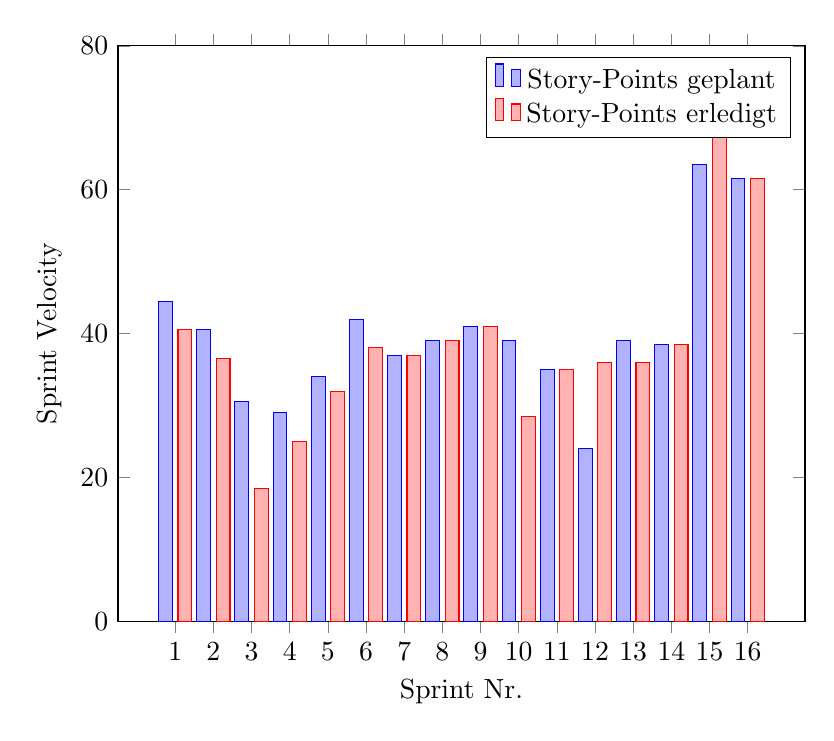
\begin{tikzpicture}
        \begin{axis}[
            ybar,
            width=0.85\textwidth,
            bar width=5pt,
            ylabel={Sprint Velocity},
            xlabel={Sprint Nr.},
            ymin=0,
            ymax=80,
            xtick=data
        ]
            \addplot[style={blue, fill=blue!30!white}] coordinates
                {(1, 44.5) (2, 40.5) (3, 30.5) (4, 29) (5, 34) (6, 42) (7, 37)
                (8, 39) (9, 41) (10, 39) (11, 35) (12, 24) (13, 39) (14, 38.5) (15, 63.5) (16, 61.5)};
            \addplot [style={red, fill=red!30!white}] coordinates
                {(1, 40.5) (2, 36.5) (3, 18.5) (4, 25) (5, 32) (6, 38) (7, 37)
                (8, 39) (9, 41) (10, 28.5) (11, 35) (12, 36) (13, 36) (14, 38.5) (15, 68.5) (16, 61.5)};
            \legend{Story-Points geplant,Story-Points erledigt}
        \end{axis}
    \end{tikzpicture}%

    \caption[Diagramm Velocity über das Projekt]{Sprint Velocity über den Verlauf des Projekts}
    \label{chart:sprint_velocity}
\end{figure}

Im Diagramm \ref{chart:sprint_velocity} ist die Sprint Velocity für jeden Sprint über den Verlauf des Projekts aufgezeichnet.
Ein Sprint dauerte jeweils eine Woche.
Zu Beginn haben wir 40 Story-Points geplant, bei jedem weiteren Sprint haben wir uns am vorherigen Sprint orientiert, wie viele Story-Points wir planen.

Ganz zu Beginn funktionierten die 40 Story-Points noch gut, aber bei Sprints 3 gab es einen Einbruch, weil wir Arbeitspakete zu gross geschätzt haben.
Dadurch wurden sie nicht innerhalb einer Woche fertig.
In den nachfolgenden Sprints konnten wir uns korrigieren und wieder auf ca. 40 Story-Points einpendeln.
Ab Sprint 12 gab es einige Einbrüche, weil andere Module gegen Ende des Semesters viel Zeit beanspruchten.
In den letzten zwei Wochen haben wir deutlich mehr Story-Points eingeplant, da das reguläre Semester vorbei war und wir uns voll auf diese Arbeit fokussieren konnten.

\subsection{Zeitauswertung}
\label{sub:Zeitauswertung}

\begin{figure}[H]
    \centering
    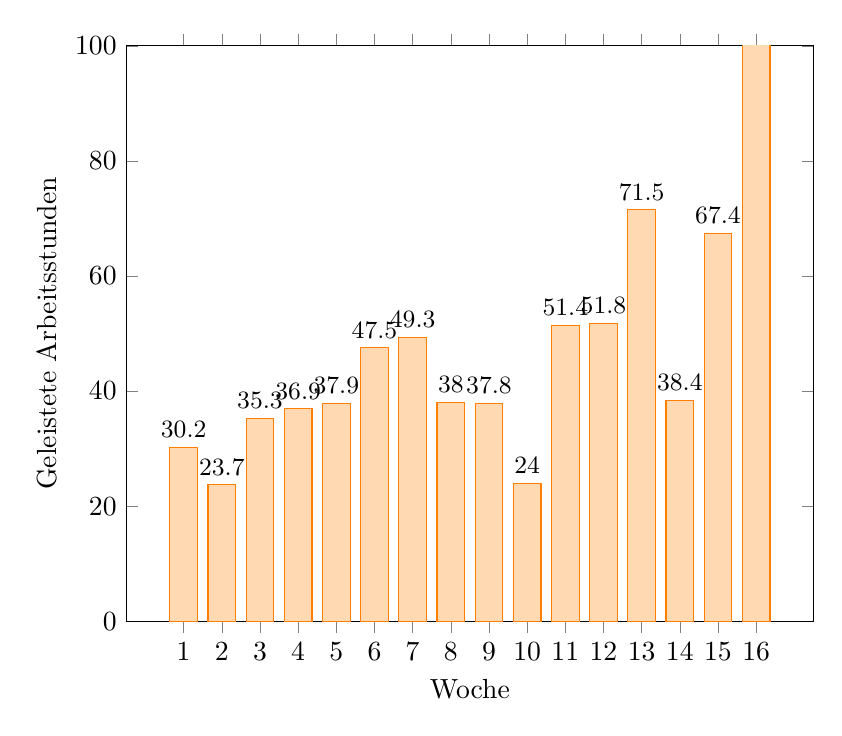
\begin{tikzpicture}
        \begin{axis}[
            ybar,
            width=0.85\textwidth,
            bar width=10pt,
            ylabel={Geleistete Arbeitsstunden},
            xlabel={Woche},
            ymin=0,
            ymax=100,
            xtick=data,
            nodes near coords,
            nodes near coords align={vertical},
            every node near coord/.append style={color=black, font=\small}
        ]
            \addplot[style={orange, fill=orange!30!white}] coordinates
                {(1, 30.2) (2, 23.7) (3, 35.3) (4, 36.9) (5, 37.9) (6, 47.5) (7, 49.3)
                (8, 38) (9, 37.8) (10, 24) (11, 51.4) (12, 51.8) (13, 71.5) (14, 38.4) (15, 67.4) (16, 105)};
        \end{axis}
    \end{tikzpicture}

    \caption[Diagramm Zeitaufwand über den Verlauf des Projekts]{Zeitaufwand über den Verlauf des Projekts}
    \label{chart:Zeitauswertung_weeks}
\end{figure}

Im Diagramm \ref{chart:Zeitauswertung_weeks} sind die geleisteten Arbeitsstunden pro Woche aufgeschlüsselt.
Der Soll-Wert des gesamten Projekts ist 720 Arbeitsstunden.
Diese sind aufgeteilt auf ca. 37 Stunden / Woche während dem Semester und 80 Stunden / Woche für die letzten zwei Wochen nach Semesterende.

In den ersten Wochen wurde weniger Arbeit als das Soll geleistet, in der Mitte konnte diese Zeit aber aufgeholt werden.
Zwischendurch gab es unregelmässige Einbrüche.
Diese sind darauf zurück zu führen, dass in diesen Wochen viel Aufwand für andere Module entstanden ist.

Insgesamt wurden bis kurz vor Abschluss \textbf{746 Arbeitsstunden} geleistet.
Die Arbeitsstunden pro Person sind mit \textbf{370 h} (Jonas Matter) und \textbf{376 h} (Robin Suter) sehr ähnlich verteilt.


\begin{figure}[H]
    \centering
    \begin{tikzpicture}
        [
            pie chart,
            slice type={admin}{piered},
            slice type={analysis}{pieyellow},
            slice type={backend}{pielblue},
            slice type={generator}{pieblue},
            slice type={infrastruktur}{pielgreen},
            slice type={thesis}{piegreen},
            slice type={webapp}{piecyan},
            slice type={specification}{piebrown},
            pie values/.style={font={\small}},
            scale=3
        ]

            \pie[xshift=2cm]{Arbeitsstunden pro Komponente}{31/generator,30/thesis,12/admin,8/webapp,6/analysis,5/specification,5/backend,3/infrastruktur}

            \legend[shift={(0cm,-1cm)}]{{OeVGK18-Generator}/generator, {Thesis}/thesis, {Administration}/admin, {Web-Applikation}/webapp}
            \legend[shift={(3cm,-1cm)}]{{Analyse}/analysis, {OeVGK18-Spezifikation}/specification, {Backend}/backend, {Infrastruktur}/infrastruktur}

        \end{tikzpicture}

    \caption[Diagramm Zeitaufwand pro Komponente]{Zeitaufwand verteilt auf einzelne Komponenten}
    \label{chart:Zeitauswertung_components}
\end{figure}

Im Diagramm \ref{chart:Zeitauswertung_components} sind die total geleisteten Arbeitsstunden auf einzelne Komponenten aufgeteilt.
Wie zu sehen ist, wurde für die Implementation des ÖV-Güteklassen 2018 Generators und das Schreiben der Arbeit jeweils rund ein Drittel der Zeit aufgewendet.